\documentclass[aps,pre,amssymb,amsmath,twocolumn,floatfix]{revtex4-2}
\usepackage{graphicx}
\usepackage{dcolumn}
\usepackage{bm}

\graphicspath{ {./img/} }
\bibliographystyle{unsrt}     %% [number]
\renewcommand{\bibname}{Bibliography}

\begin{document}

\title{[NO NAME ARTICLE]}

\author{Ilya Pchelintsev}
\author{Kamilla Faizullina}
\author{Evgeni Burovski}
\affiliation{HSE University, 101000 Moscow, Russia}


% абстракт и введение я напишу немного позже, когда будет более полное
% осмысление работы

\begin{abstract}
    This is an abstract and that's really abstract.
\end{abstract}

\maketitle

\section{Introduction}
This is cite-checking.\cite{Papale2018}

\section{Models and Methods}
In the paper we consider several models: the first one is Ising model on interacting self-avoiding walk from the [REF KAMILLA], on three different lattices: 2D-square lattice, 3D-square lattice and 2D-triangle lattice. The main difference between square and triangle lattice in defining two additional diagonal monomers on lattice as nearest too, see [FIGURE FOR 2D-SQUARE AND 2D-TRIANGLE LATTICE]. Considering the case of lack of outer magnetic field in this work, the Hamiltonian of the model of fixed conformation $u$ with length $N$ and strength of nearest-neighbors interaction $J$ reads:

% здесь я хочу добавить два рисунка для квадратной и треугольной решёток -
% чтобы было видно, какие связи и по какой диагонали были добавлены 

\begin{equation}\label{H_Ising_ISAW}
  H_{u, N, \{\sigma\}} = - \sum_{\langle i,j \rangle} J  \sigma_{i}  \sigma_{j},\ \ i,j \in u,\ |u| = N
\end{equation}

The summation runs through spins involved in conformation and only with the nearest neighbors. 

The second model considered in this paper is the Ising model on the rectangular lattice from the [REF SELKE]. Simulated lattices has $L \times rL$ spins and the Hamiltonian is calculated through interaction between all spins and their nearest neighbors respectively:

\begin{equation}\label{H_Ising_Rectan}
  H_{L, r, \{\sigma\}} = - \sum_{\langle i,j \rangle} J  \sigma_{i}  \sigma_{j},\ \ i,j \in [1..L] \times [1..rL]
\end{equation}

% Здесь я добавлю описание третьей модели, обычного SAW,
% просто пока не успел

For comparing magnetic properties of models with similar geometric ones we also define shape factors, such as gyration tensor [REF PELLISETTO]:

\begin{equation}\label{eq:Ten_G1}
    Q_{N,\alpha\beta} = \frac{1}{N+1} \sum^{N}_{i=0}(w_{i,\alpha} - w_{c, \alpha})(w_{i,\beta} - w_{c, \beta})
\end{equation}

where $N$ is length of the system (number of monomers in conformations of Ising-ISAW models and number of spins in the lattice in rectangular Ising), and  $\alpha,\beta$ are coordinates (so, $Q_{N, xx}$ and $Q_{N,yy}$ can be defined as mean squares of coordinates of the points of the model in the cartesian coordinate system with the center in the center of model). Eugen values $q1$, $q2$ of given tensor can be interpreted as $Q_{N, xx}$ and $Q_{N,yy}$ in the coordinate system of eugen vectors, or more important - as square of semi-axes of ellipse of inertia of given system. The proportion of them for systems with length $N$ will be[REF PELLISSETTO]: 

\begin{equation}
    r = \sqrt{\frac{\langle q_{1}\rangle_{N}}{\langle q_{2} \rangle_{N}}}
\end{equation}

Eugen values $q1$, $q2$ are also used in enumerating another important shape factor - mean asphericity[REF PELLISETTO]:

\begin{equation}
\label{eq:Asphericity}
    \mathcal{A} = \left\langle \frac{(q_{1} - q_{2})^{2}}{(q_{1} + q_{2})^{2}} \right\rangle_{N}
\end{equation}

% Здесь хочу добавить два графика - прямоугольника и случайного блуждания
% с соответствующими им эллипсами инерции - попробую сделать так чтобы они
% имели одинаковую асферичность - чтобы была ясна задумка первого сюжета

The compared magnetic property of our models is the fourth order cumulant of the magnetization of the Binder cumulant, defined as[REF SELKE]:

\begin{equation}
\label{eq:Cumulant}
U_{4} = 1 - \frac{\langle m^{4} \rangle}{3 \langle m^{2} \rangle^{2}}
\end{equation}

Where $\langle m^{4} \rangle$ and $\langle m^{2} \rangle$ are mean fourth and second order of mean magnetization per spin respectively.

We also need to define mean proportion of monomers with fixed number $i$ of nearest neighbors $\langle n_{i} \rangle$, which is counted directly for every monomer in every simulated conformation of walk.

We are interested in comparing models in their respective critical regions. For each structure, critical temperatures of Ising models are known as[REF FOSTER][REF SELKE]:

\begin{table}[h]
    \centering
    \begin{tabular}{|c|c|c|}
        \hline
        Type of lattice & $T_{c}$ \\ \hline
        2D-square & $1.199 \pm 0.003$ \\ \hline
        3D-square & $1.90 \pm 0.02$\\ \hline
        Rectangular & 2.26918...\\ \hline
    \end{tabular}
    \caption{Known values of critical temperature of different modifications of Ising-ISAW model and normal Ising on the rectangular lattice}
    \label{tab:my_label}
\end{table}

% сюда немного позже добавлю критические значения для модели SAW

\textit{Method.} All methods of simulating for Ising model on a SAW conformation are remained the same as in[REF KAMILLA]. For simulating Rectangular Ising, however, we used cluster update of Wolff Algorithm[REF NEWMAN BARKEMA][REF SCHRODINGER CAT].

% Стоит ли добавлять рисунок шага алгоритма 
% и более подробное объяснение методов?? Поскольку ничего не было добавлено, % я решил не расписывать, но описание методов получилось крайне немногословным))


% на самом деле, мне ещё не до конца понятно, какую часть теории достаточно
% просто добавить ссылкой, а что лучше добавить подробным разъяснением

\section{Results}

\subsection{Mean Asphericity and Critical Cumulant}

% если я правильно понимаю, данную подсекцию можно полностью взять из отчёта
% (9.6), как раз данная часть больше всего похожа по содержанию на Results -
% план действий (какие длины были взяты, под какую модель и т.д.), описания
% графиков, таблицы; только с заключением вопрос - его стоит добавить в 
% условный Conclusions или рассужждения о результате желательны здесь же 
% перед частью Bulk.

%пока только рисунки, для хронологии
%более подробное объяснение добавлю позже

We attempted to learn how magnetic properties of Ising-like models depend on their geometrical ones and to define their comparability in critical region, where observable values of models don't depend on the length of conformation $N$. As we know, in the Ising model on rectangular lattice shape factors like aspect ratio $r$ are the parameters, not observable values. Therefore, we can find value of asphericity $\mathcal{A}$ for any aspect ratio.

\begin{figure}[h]
    \centering
    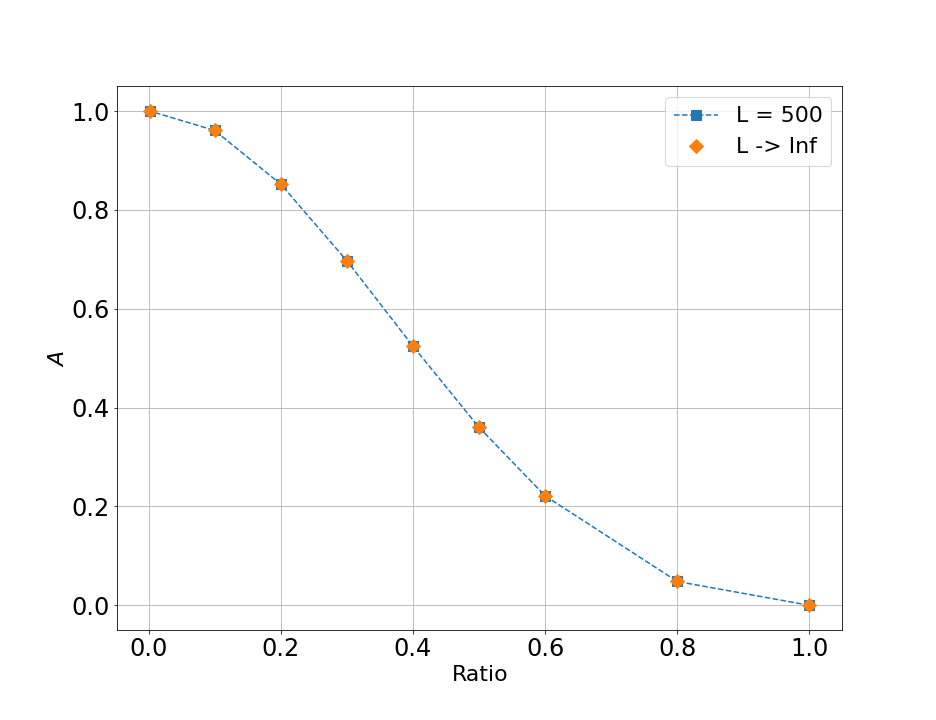
\includegraphics[width=\columnwidth]{Images/A_r.png}
    \caption{Asphericity as function of aspect ratio $r$ of the rectangular lattice}
    \label{fig:A_r}
\end{figure}

% следует ли добавить расчёты оценки зависимости асферичности 
% прямоугольника от стороны? Или это лучше добавить в models and methods?

 We found values of aspericity of Ising-ISAW and ISAW models in their respective critical regions. They are used to enumerate aspect ratio of the rectangular lattice with the same value of asphericity.

\begin{figure}[h]
    \centering
    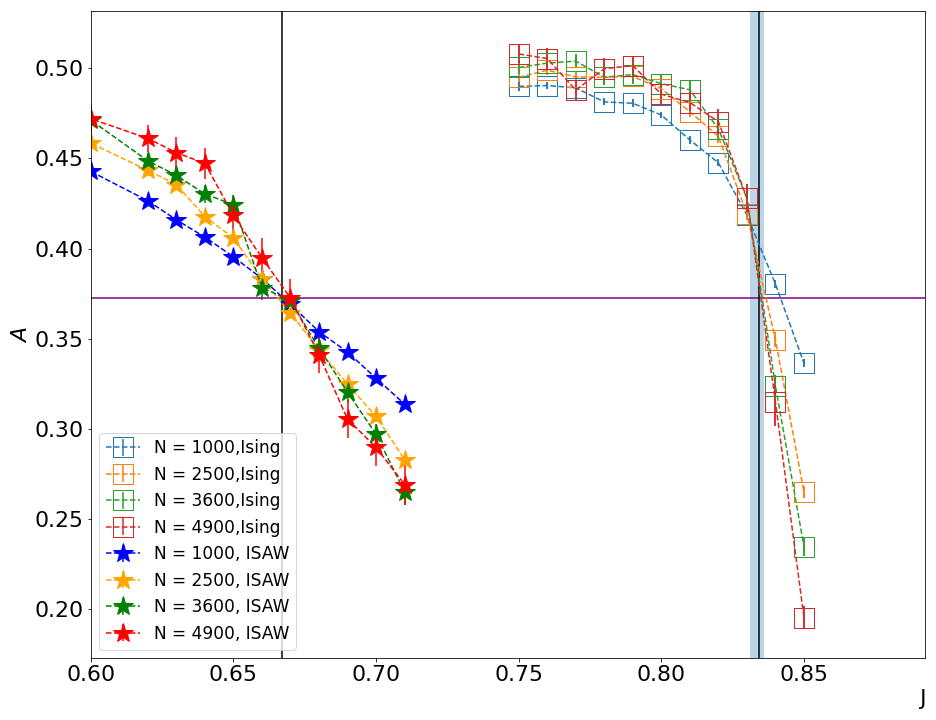
\includegraphics[width=\columnwidth]{Images/Ising_ISAW_A_J_Full.png}
    \caption{Asphericity of Ising-ISAW (empty squares) and ISAW-only models (stars) as function of $J=1/T$, varying lengths of conformations $N$ = 1000 (blue), 2500 (yellow), 3600 (green) and 4900 (red)}
    \label{fig:Ising&ISAW_A_J}
\end{figure}

\begin{figure}[h]
    \centering
    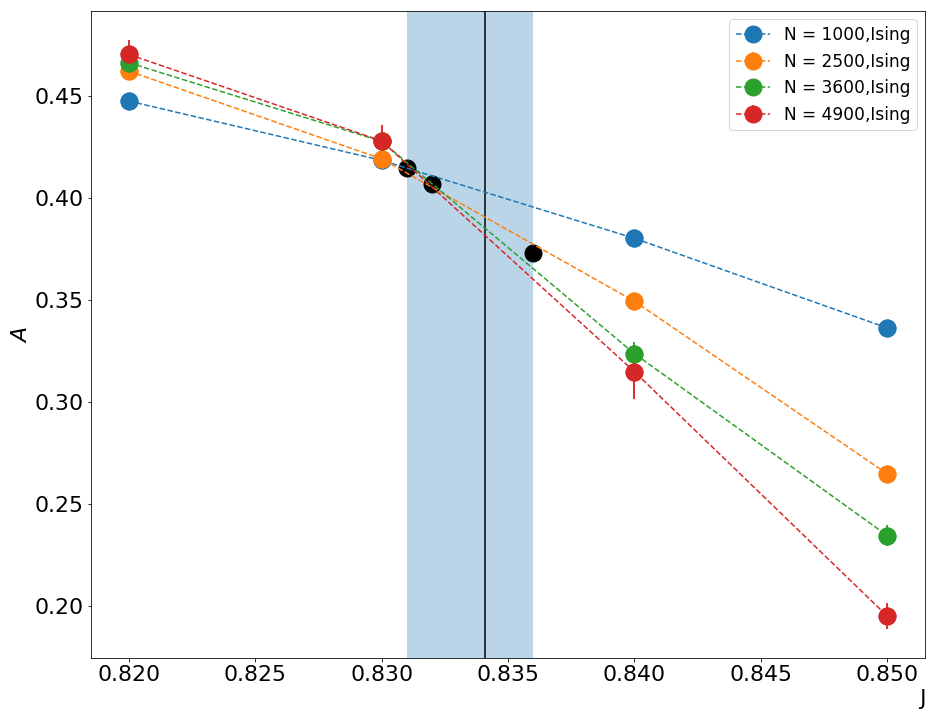
\includegraphics[width=\columnwidth]{Images/Ising_A_J_Close.png}
    \caption{Asphericity of Ising-ISAW model as function of zoomed in the critical region (red vertical lines), varying lengths of conformations N = 1000 (blue), 2500 (yellow), 3600 (green) and 4900 (red)}
    \label{fig:Ising_A_J}
\end{figure}

\begin{figure}[h]
    \centering
    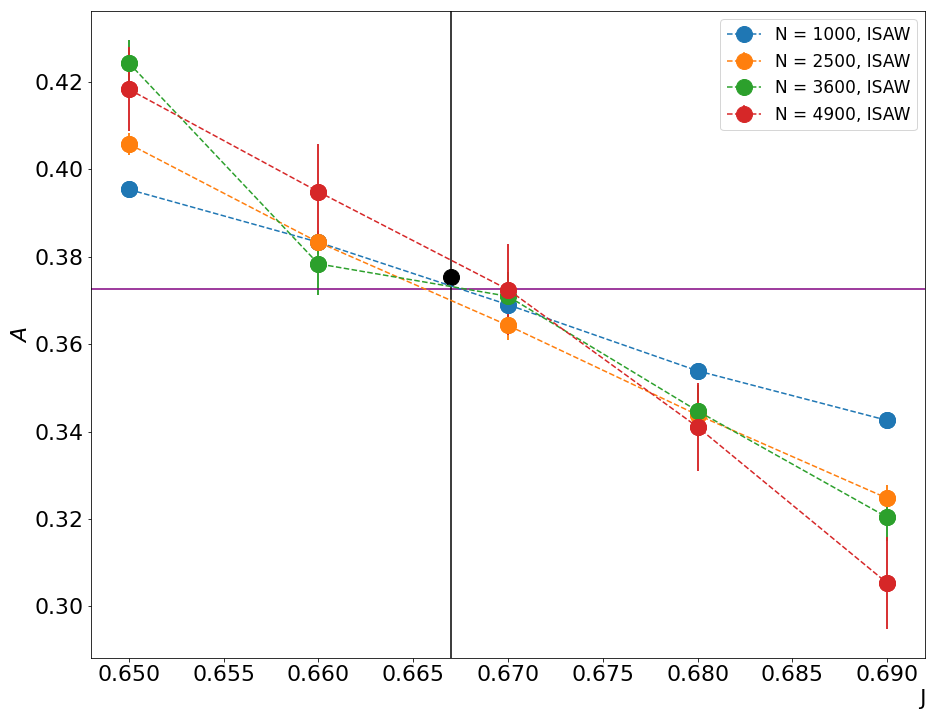
\includegraphics[width=\columnwidth]{Images/ISAW_A_J_Close.png}
    \caption{Asphericity of ISAW model as function of zoomed in the critical region (red vertical lines), varying lengths of conformations N = 1000 (blue), 2500 (yellow), 3600 (green) and 4900 (red)}
    \label{fig:ISAW_A_J}
\end{figure}

\begin{table}[h!]
    \centering
    \begin{tabular}{|c|c|c|c|}
        \hline
         \multicolumn{4}{|c|}{PolIsing}  \\ \hline
         J & $\mathcal{A}$ & r & $U_{4}\  Rectangular$ \\ \hline
         0.831 & 0.415 & 0.465 & $0.340 \pm 0.006$\\ \hline
         0.832 & 0.4072 & 0.47 & $0.343 \pm 0.006$\\ \hline
         0.836 & 0.373 & $0.490 \pm 0.002$ & $0.348 \pm 0.006$\\ \hline
         \multicolumn{4}{|c|}{ISAW} \\ \hline
         0.667 & 0.375 & 0.49 & $0.349 \pm 0.006$ \\ \hline
    \end{tabular}
    \caption{Values of critical cumulant for Ising model on rectangular lattice with mean asphericity related to models ISAW and Ising-ISAW in their critical regions}
    \label{tab:A_r_U}
\end{table}

\subsection{Bulk}

\section{Discussion}

\section{Acknowledgments}

\bibliography{bibliography}

\end{document}